\documentclass[]{article}
\usepackage[utf8]{inputenc}
\usepackage[italian]{babel}
\usepackage[a4paper,left=2cm, right=2cm]{geometry}
\usepackage{amsmath}
\usepackage{amssymb}
\usepackage{graphicx}
\usepackage[bottom]{footmisc}

\begin{document}
\newcommand{\campo}[1]{\mathbb{#1}}

\title{Relazione Progetto Simple Social}
\author{Alessandro Pagiaro}
\date{\today}
\maketitle
\tableofcontents
	\pagebreak
\section{Descrizione del progetto}
Il progetto si divide in tre package:
\begin{itemize}
	\item SocialServer: contiene tutto ciò che riguarda il server
	\item SocialClient: contiene tutto ciò che riguarda il client
	\item SimpleSocial: contiene le strutture condivise tra client e server, le eccezioni e le classi dei messaggi scambiati
\end{itemize}

Si forniscono di appendice i diagrammi delle classi del Client e del Server

\section{Comunicazione}
\subsection{Protocollo di comunicazione}
	Lo scambio di messaggi avviene tramite oggetti di tipo \texttt{PacketMessage} che vengono serializzati e quindi spediti. Per l'invio ogni \texttt{PacketMessage} viene serializzato su un \texttt{ByteArrayOutputStream}, si legge quindi la dimensione e viene scritta nella socket. Il ricevente legge i primi 4 byte, alloca un buffer delle dimensioni segnate in quei 4 byte (= int) e quindi legge i byte dell'oggetto. Al termine lo deserializza e lo passa al livello sovrastante.
	
	Il \texttt{PacketMessage} al suo interno contiene un valore \textit{type} che indica il tipo del messaggio contenuto al suo interno e un \textit{message} che riferisce il \texttt{SimpleMessage}.
\subsection{Server}
Il server lavora tramite NIO, ricevendo i messaggi sui vari channel. Ogni \textit{key} ha un attachment che contiene i dati ricevuti e ne tiene il conto al fine di eseguire il protocollo di serializzazione e derializzazione sopra descritto. Ogni pacchetto, una volta ricevuto completamente, viene passato al livello successivo (rappresentato dal MainServer) che avvia un thread \footnote{Con eccezione dei messaggi riguardanti lo scambio di richieste di amicizia che poichè devono andare a registrare un nuova channel al selettore non possono che essere gestiti nello stesso thread per evitare situazioni di attesa indeterminata dovuta a lock implicite del selettore} che gestisce la richiesta e imposta anche il messaggio di risposta da mandare al client \footnote{A differenza delle richieste di amicizia, negli altri casi viene usata sempre la stessa \textit{key}, andando a modificare le \textit{interestedOps}, operazione che risulta thread-safe}
L'attachment di ogni \textit{key} è di tipo \texttt{ObjectSocketChannel}.

\subsection{Client}
Il client lavora in maniera più semplice rispetto al server. Utilizza le normali socket con chiamate bloccanti. Il protocollo di lettura e scrittura sopra descritto è attuato tramite l'oggetto \texttt{ObjectSocket \textit{extends} Socket} che ridefinisce le funzioni \textit{write()} e \textit{read()}.
\subsubsection{\texttt{Listener}}
Il client all'avvio crea un thread che si mette in ascolto su una porta casuale che verrà comunicata al server al momento del login. Tale thread gestirà le nuove richieste di amicizia in entrata ed \textbf{non} sostituisce la funzione RMI di callback per la pubblicazione dei contenuti.

\subsection{KeepAlive}
Il KeepAlive (da ora KA) viene gestito dal server tramite due thread creati all'avvio e definiti nel file \textit{KeepAliveServerService} \footnote{Un thread è dichiarato inline nel file stesso}. Mentre un thread spedisce un messaggio ogni KEEP\_ALIVE\_DELAY (vedere sezione \ref{param}) e si preoccupa dopo 10 secondi di rimuovere i client che non hanno effettuato iterazioni, l'altro thread ha il compito di ricevere le risposte KA e segnalare in una lista contenuta in \texttt{UserDB} l'avvenuta iterazione. Da notare che anche se il pacchetto viene perso (viaggia infatti su UDP), se l'utente effettua una connessione per qualsiasi altra iterazione con il server, questa viene segnalata e quindi non finirà offline non avendo risposto al KA perchè comunque una iterazione è avvenuta.

\section{Parametri e costanti} \label{param}
Le costanti sono caricate dinamicamente all'avvio sia nel client che nel server. Il server utilizza il file \texttt{config.txt}, mentre il client utilizza il file \texttt{client\_config.txt}. Entrambi i file devono essere contenuti nelle rispettive working directory.

\section{Salvataggio dei dati nel server}
In caso di crash il server è in grado di ricostruire il proprio database. Difatti ad ogni evento fondamentale (aggiunta di un utente, richieste di amicizia, follower...) viene serializzato il database (pulito di liste temporanee come ad esempio la lista degli utenti online) su file. Tale file viene caricato dinamicamente all'avvio. 

\section{Appendice}
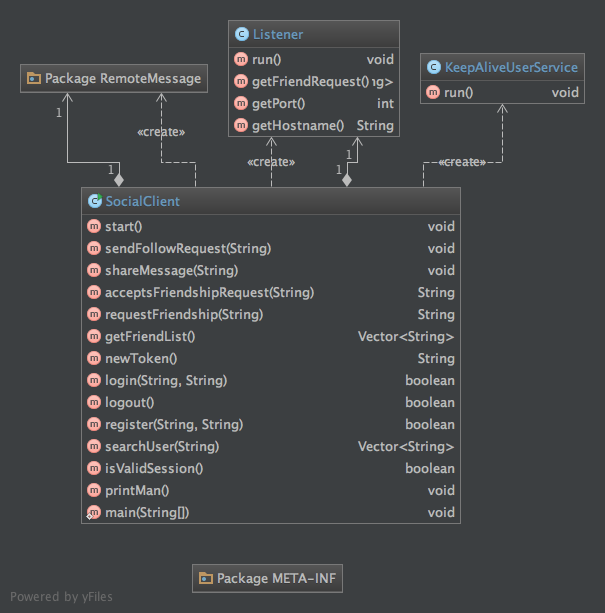
\includegraphics[width=\linewidth]{Client}

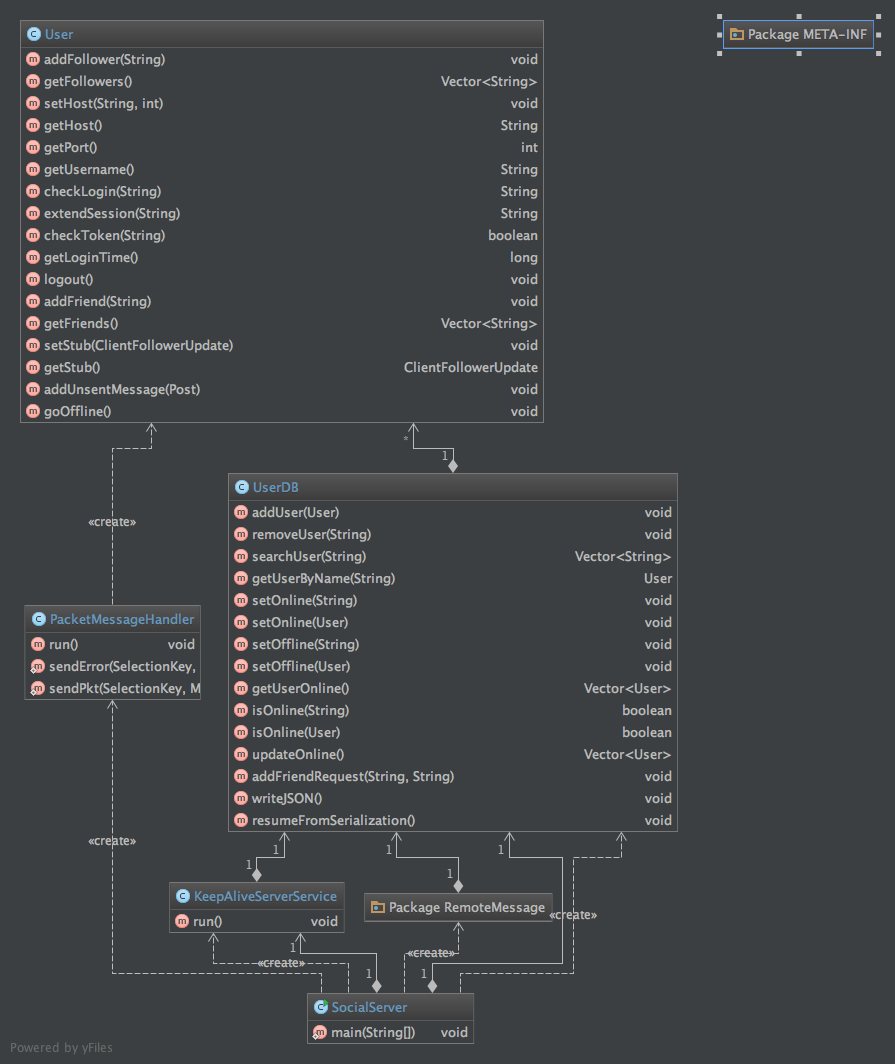
\includegraphics[width=\linewidth]{Server}



\end{document}